\documentclass{beamer}
\usepackage{graphicx}
\usepackage{amssymb,amsfonts,amsmath}
% \usepackage{tikz,tkz-euclide}
% \usepackage{subfigure}
% \usepackage{parskip}
% \usetikzlibrary{arrows.meta}
% \usetikzlibrary{calc,patterns}
\usefonttheme[onlymath]{serif}
% \usetheme{Berlin}
\title{Weekly Report}
\author{WU Zihan}
\begin{document}
\maketitle
% \begin{frame}
%     \frametitle{Outline}
%     \tableofcontents
% \end{frame}

\section{Introduction}
\begin{frame}
    \frametitle{Applcation}
    \begin{itemize}
        \item Industrial Yield Prediction
        \item Calibration of Lens
    \end{itemize}
\end{frame}

\begin{frame}
    \frametitle{Result}

    % 1. constrain on long axis, short axis, and eccentricity (abande.png)
    % 2. constrain more on angle (moreonangle.png)

    % columns
    \begin{columns}
        \column{0.5\textwidth}
        \begin{figure}
            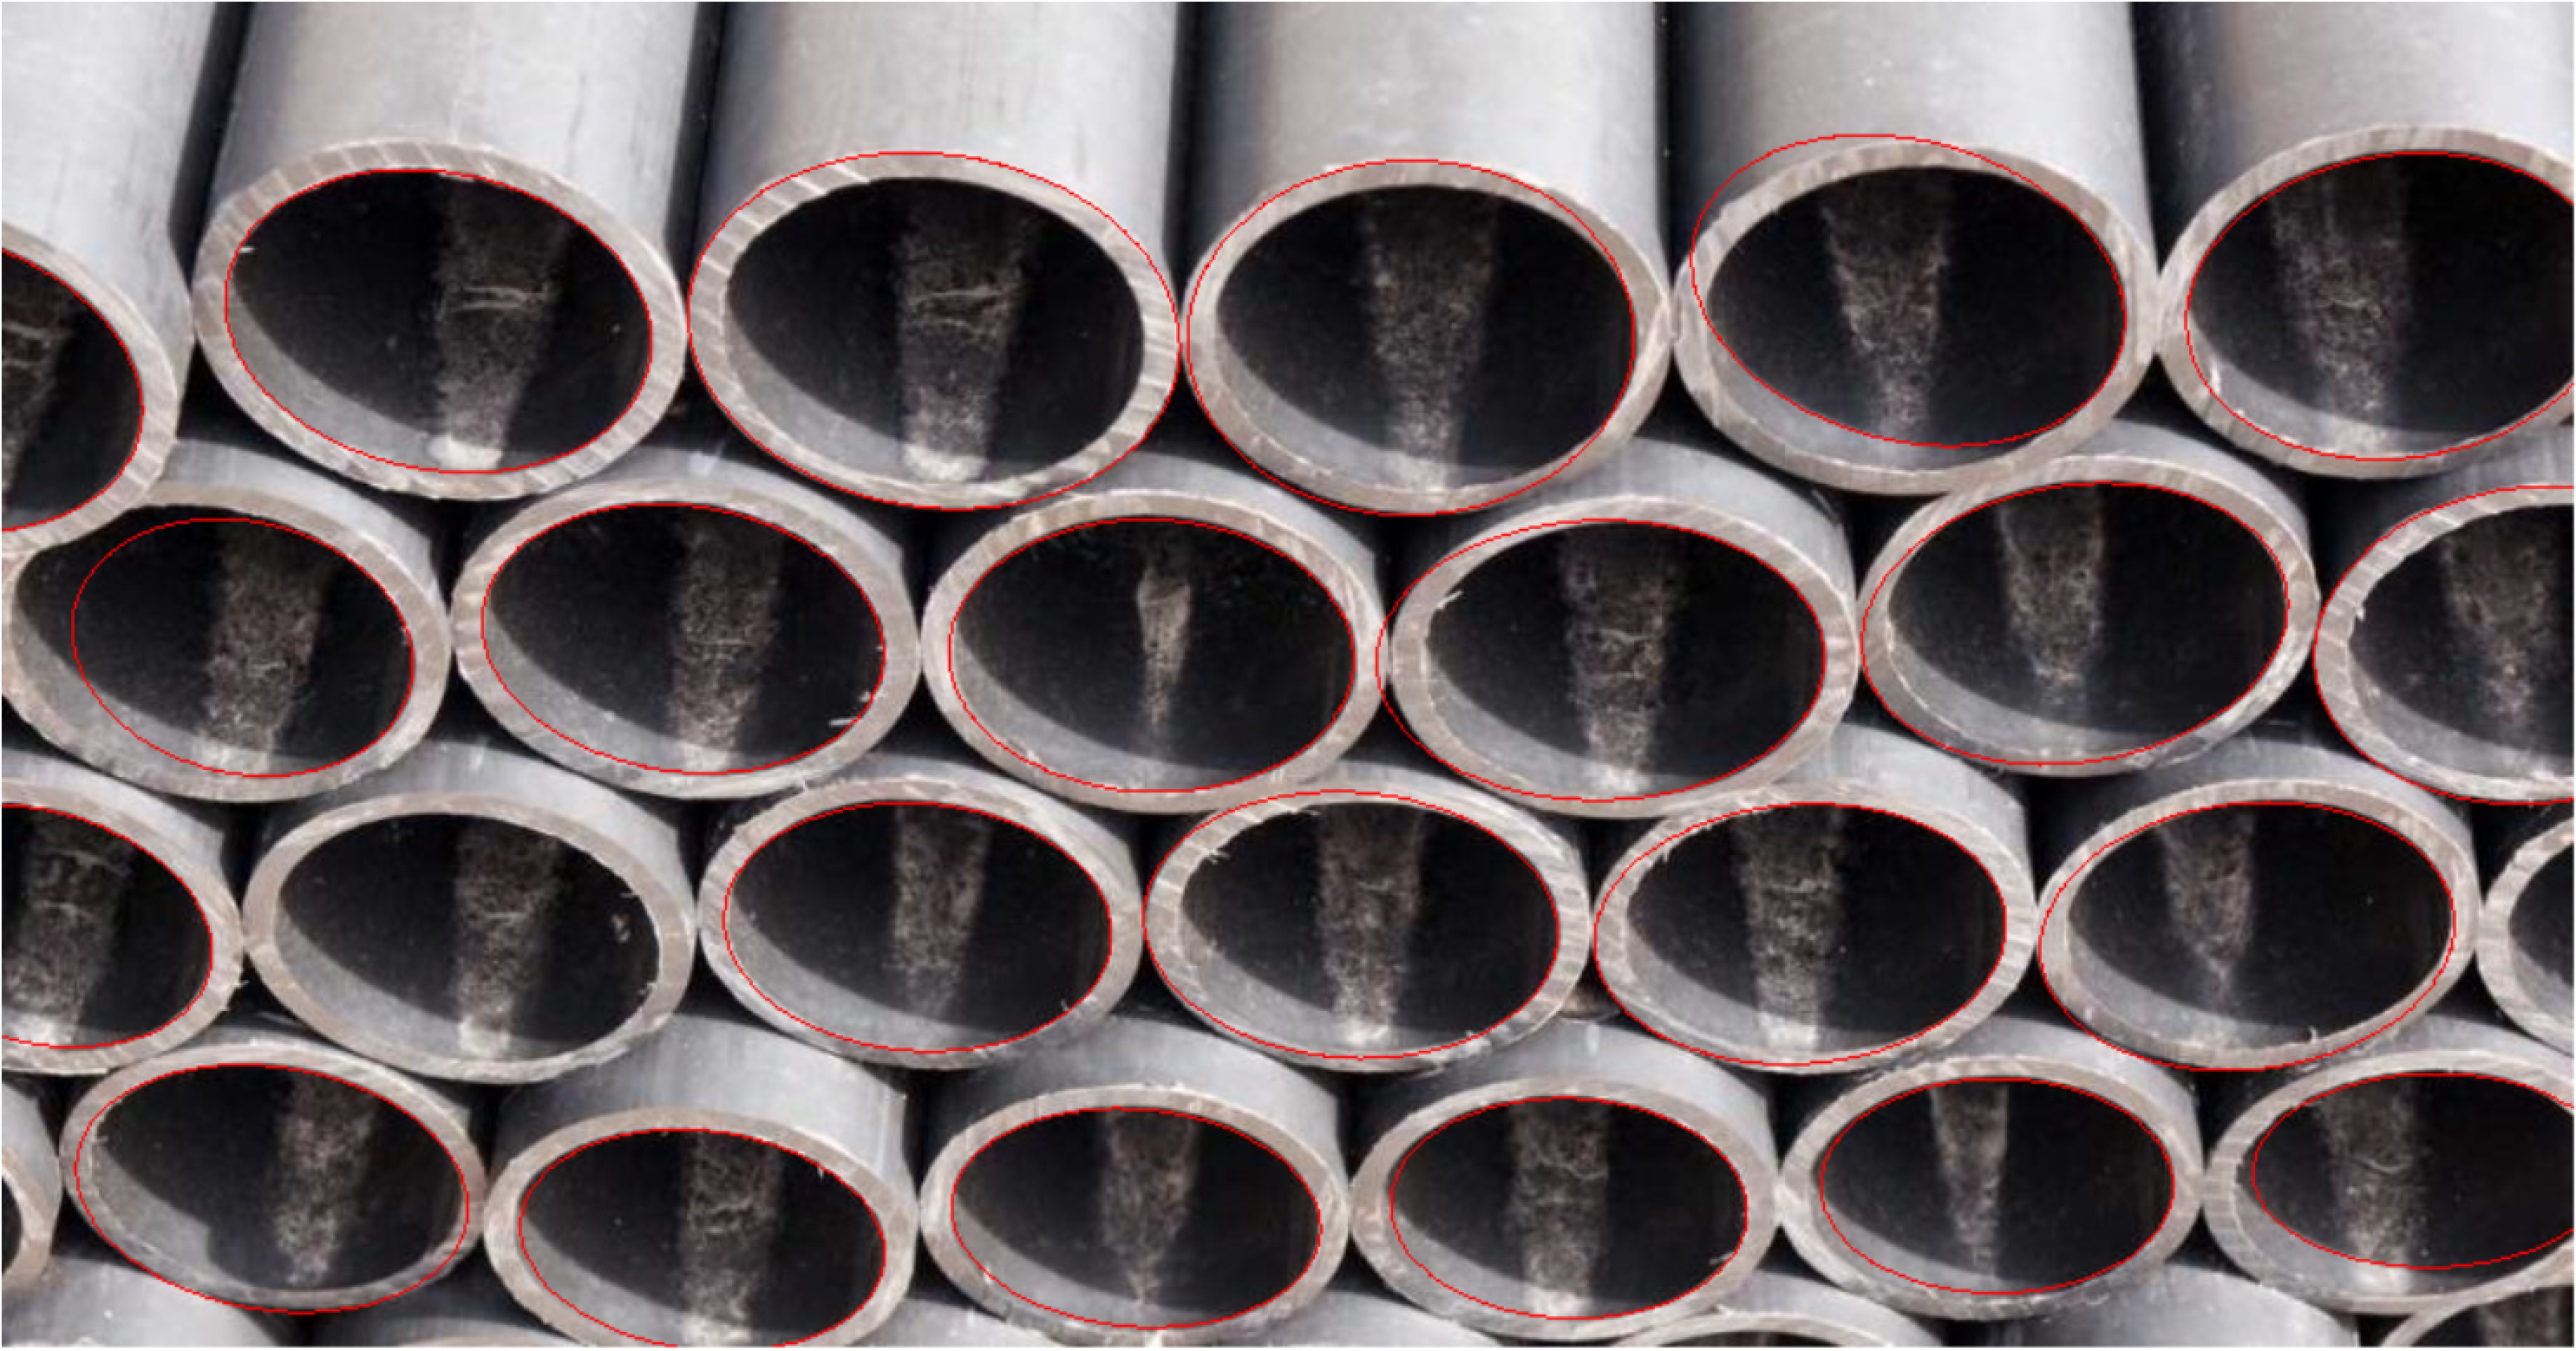
\includegraphics[width=\textwidth]{abande.png}
            \caption{Constrain on long axis, short axis, and eccentricity}
        \end{figure}
        \column{0.5\textwidth}
        \begin{figure}
            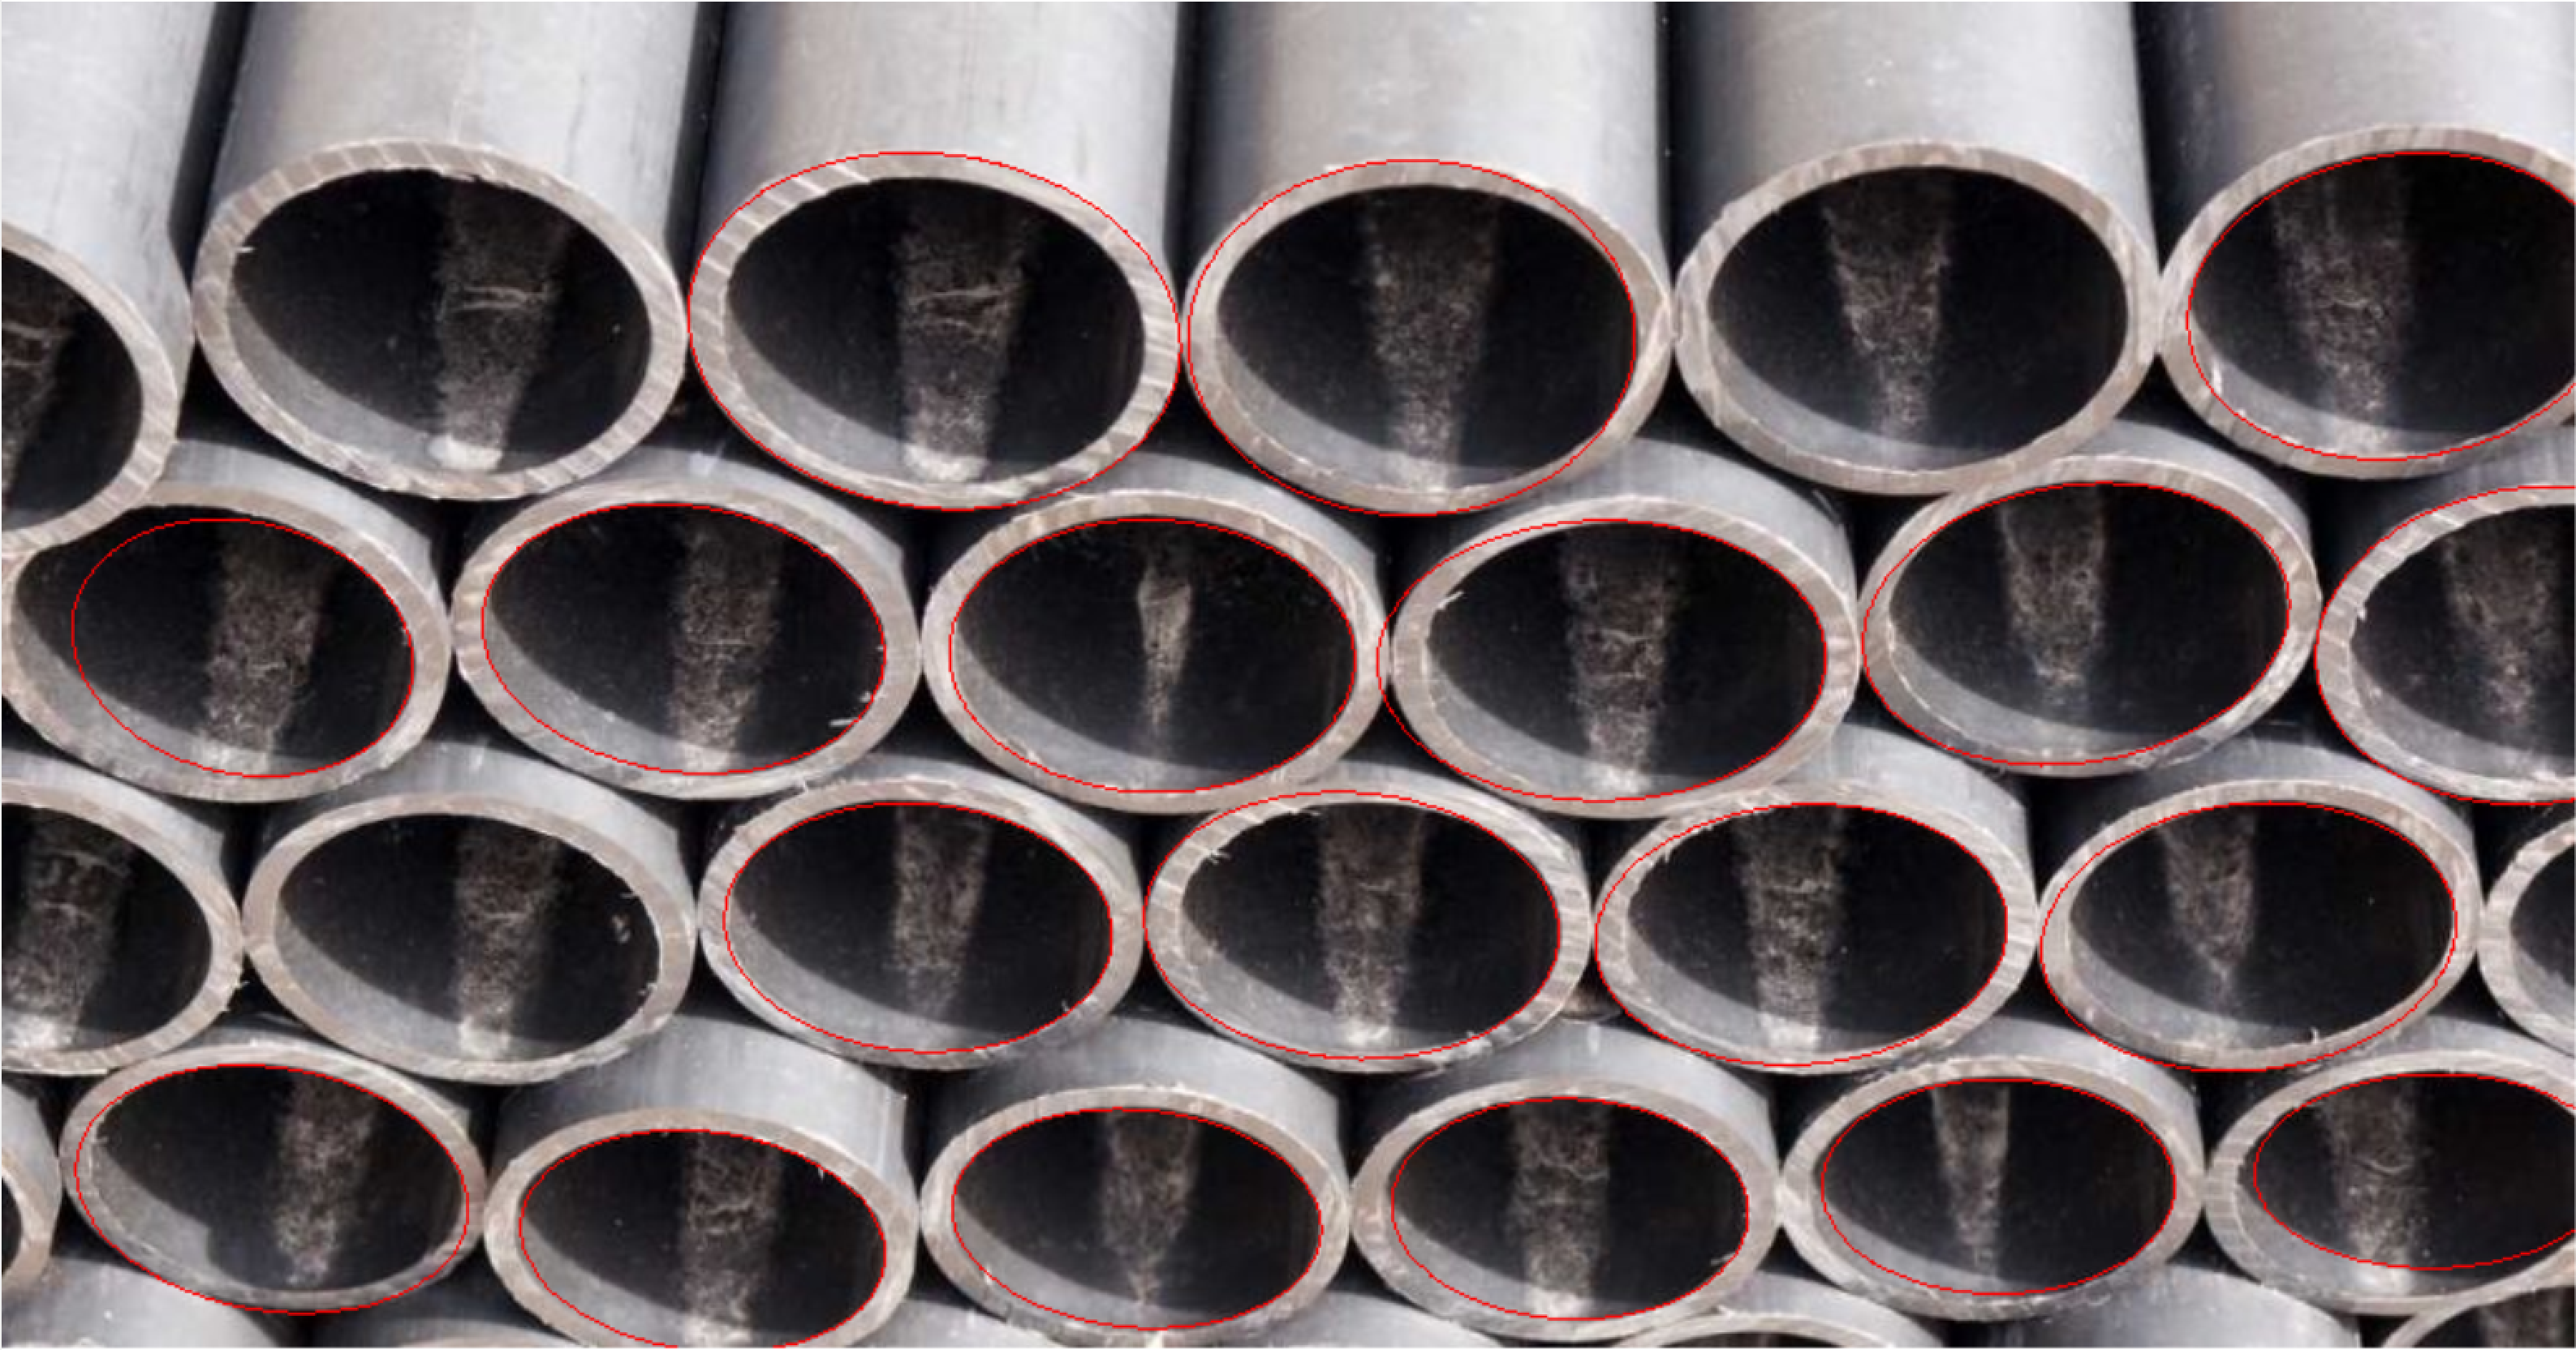
\includegraphics[width=\textwidth]{moreonangle.png}
            \caption{Constrain more on angle}
        \end{figure}
    \end{columns}

    

\end{frame}

\end{document}